\subsection{\name{YuvKA.VideoModel}}

\subsubsection*{Aktuelles Klassendiagramm}
\begin{figure}[h!]
\begin{center}
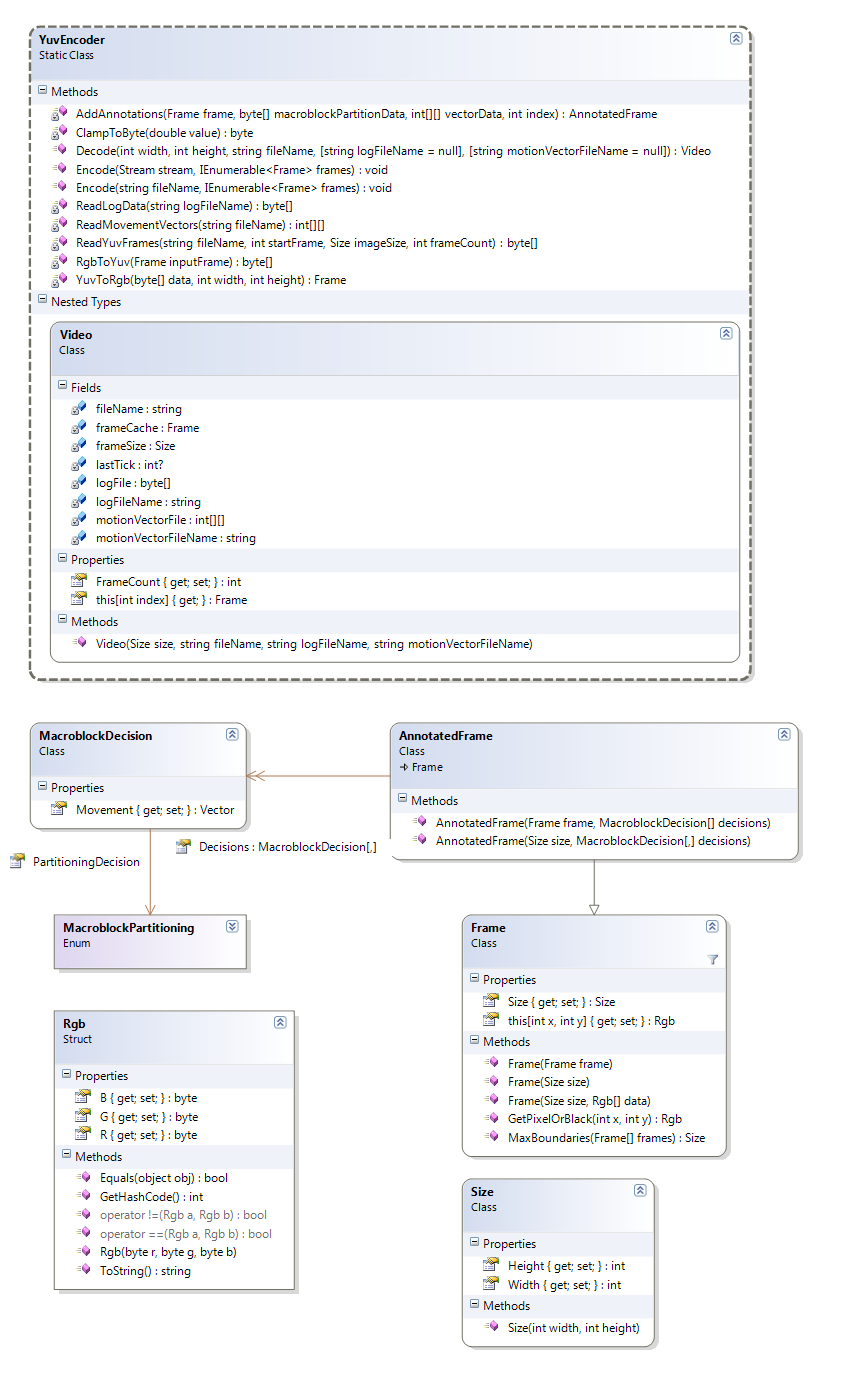
\includegraphics[height=0.7\textheight]{classdiagram/videomodel.png}
\end{center}
\end{figure}
Das VideoModel repräsentiert ein eingelesenes Video, ggf. mit zugehörigen Log-Daten. Da es die Daten im RGB-Format speichert, müssen diese bei Eingabe und Ausgabe von einem YUV-Encoder konvertiert werden.
\newpage

\paragraph{\name{Frame}}
\begin{itemize}
	\add \verb!public  GetPixelOrBlack(int x, int y)! \\
	Neue öffentliche Methode, die es erleichtern soll, auf die Farbwerte eines Frames zuzugreifen. Es muss nicht mehr beachtet werden, ob die gegebenen Koordinaten tatsächlich innerhalb des \name{Frame} liegen. Falls dies der Fall ist, so wird der entsprechende Pixel an Stelle (x, y) als \name{Rgb}-Objekt zurückgegeben. Falls nicht, so wird ein schwarzer Farbwert für den Pixel zurückgegeben.
	\add \verb!public MaxBoundaries(Frame[] frames)! \\
	Neue öffentliche Methode, welche aus einem Array von Frames jeweils das Maximum der Breite und der Höhe findet und ein \name{Size}-Objekt mit ausreichend großen Werten zurückgibt.
\end{itemize}

\paragraph{\name{MacroblockDecision}}
\begin{itemize}
	\change \verb!public Vector Movement { get; set; }! \\
	Die \name{Movement}-Property wurde schreibbar gemacht, da eine korrekte Initialisierung sonst nicht möglich wäre.
	\change \verb!public MacroblockPartitioning? PartitionDecision { get; set; }! \\
	Die \name{PartitionDecision}-Property wurde schreibbar gemacht, da eine korrekte Initialisierung sonst nicht möglich wäre.
\end{itemize}

\paragraph{\name{Rgb}}
\begin{itemize}
	\change \verb!public byte R { get; }! \\
	Der Setter der R-Property wurde auf private gesetzt.
	\change \verb!public byte G { get; }! \\
	Der Setter der G-Property wurde auf private gesetzt.
	\change \verb!public byte B { get; }! \\
	Der Setter der B-Property wurde auf private gesetzt.
\end{itemize}

\paragraph{\name{YuvEncoder}}
\begin{itemize}
	\add \begin{verbatim}public static Video Decode(int width, int height,
	    string filename, string logFileName = null,
	    string motionVectorFileName = null)
		\end{verbatim}
	Neuer Parameter: \verb!string motionVectorFileName = null!\\
	Die an ein Video gebundenen Bewegungsvektoren sollen schon beim Lesen eines Videos vom Hintergrundspeicher gelesen werden, da \name{Video}-Obekte unveränderlich sind, und bei Neuwahl der entsprechenden Datei ein neues Video-Objekt erstellt werden muss.
	\add \begin{verbatim}public static void Encode(Stream stream, 
	    IEnumerable<Frame> frames)
	\end{verbatim}
	Neue öffentliche statische Methode Encode, welche als Parameter einen Stream entgegennimmt. Dies ermöglicht es, zu Testzwecken auch in einen \name{MemoryStream} zu schreiben, was den Hintergrundspeicher nicht belastet und in der Regel schneller ist.
\end{itemize}

\paragraph{\name{YuvEncoder.Video}}
\begin{itemize}
	\remove \verb!public void Dispose()! \\
	Da keine Streams länger als unbedingt nötig offen gehalten werden, wird die zuvor von der \name{Video}-Klasse implementierte Schnittstelle \name{IDisposable} hier nicht mehr benötigt. Dadurch entfällt diese Methode.
\end{itemize}
\newpage

\subsection{\name{YuvKA.Pipeline}}

\subsubsection*{Aktuelles Klassendiagramm}
\begin{figure}[h!]
\begin{center}
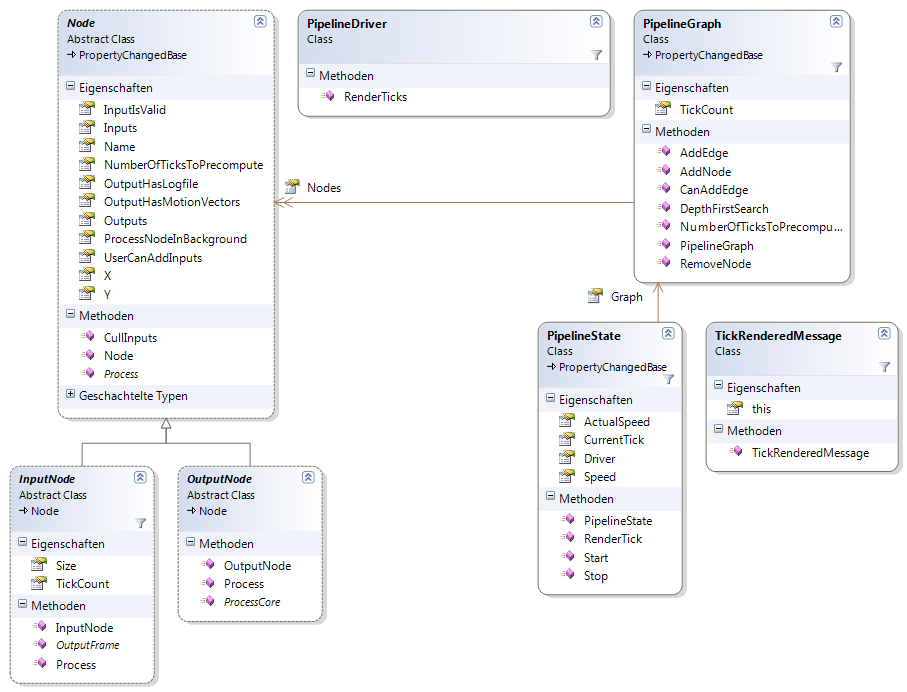
\includegraphics[width=\textwidth]{classdiagram/pipe.png}
\end{center}
\end{figure}
Die Pipeline-Schicht repräsentiert den UI-unabhängigen Aufbau des Analyse-DAGs\footnote{\emph{directed acyclic graph}}. Sie besteht einerseits aus den unterschiedlichen Knoten-Klassen, die unabhängig voneinander ihren jeweiligen Algorithmus auf Frame-für-Frame-Basis implementieren, und andererseits aus dem Pipeline Driver, der für die Abhängigkeitsauflösung und letztendliche Abarbeitung der Pipeline zuständig ist.
\newpage

\paragraph{\name{InputNode}}
\begin{itemize}
	\change \verb!public int? TickCount { get; }! \\
	Die Property \verb!TickCount! ist nun nullable. Der Wert null steht hierbei für die Möglichkeit beliebig viele Frames zu erzeugen.
\end{itemize}

\paragraph{\name{Node}}
\begin{itemize}
	\change \verb!public Node(int? inputCount, int? outputCount)! \\
	Die Parameter des Konstruktors sind jetzt nullable, um mit dem Wert null eine variable Anzahl von Ein-/Ausgängen zu repräsentieren.
	\add \verb!public virtual bool InputIsValid { get; }! \\
	Diese Property wurde eingeführt, um repräsentieren zu können, ob alle Inputs des Knotens (indirekt) mit validen InputNodes verbunden sind und der Knoten somit seine Berechnung auch ausführen kann.
	\add \verb!public string Name { get; set; }! \\
	Repräsentiert den Namen des Knoten. Der Name eines Knoten ist eine möglichst kurze Beschreibung der Funktionsweise des Knotens. Im Idealfall ist diese Beschreibung nur ein Wort lang.
	\add \verb!public virtual int NumberOfFramesToPrecompute { get; }! \\
	Wurde eingeführt, da manche Knoten Daten aus vergangenen Ticks zur Berechnung des aktuellen Ticks brauchen. Damit diese Knoten auch nach dem Springen in der Pipeline das korrekte Ergebnis liefern, muss man eventuell Ticks vorberechnen. Diese Property repräsentiert, wie viele vergangene Frames der Knoten kennen muss, um seine Berechnung auszuführen.
	\add \verb!public virtual bool OutputHasLogfile { get; }! \\
	Wurde eingeführt, um repräsentieren zu können, ob die Ausgabe des Knotens Logfiles beinhaltet.
	\add \verb!public virtual bool OutputHasMovementVectors { get; }! \\
	Wurde eingeführt, um repräsentieren zu können, ob die Ausgabe Movement-Vektoren beinhaltet.
	\add \verb!public virtual bool UserCanAddInputs { get; }! \\
	Diese Property gibt an, ob der User in der Lage sein soll Inputs zu diesem Knoten hinzuzufügen.
	\add \verb!public void CullInputs()! \\
	Diese Methode wurde eingeführt, um eventuell unnötige Eingänge eines Knotens zu entfernen.
	\remove \verb!public void Dispose()! \\
	Die Methode \verb!Dispose()! wurde entfernt, da keine Streams mehr offen gehalten werden.
\end{itemize}

\paragraph{\name{Node.Input}}
\begin{itemize}
	\remove \verb!public int Index { get; }! \\
	Wurde entfernt, da es nicht mehr gebraucht wurde und Node.Input keinen Zugriff auf seinen Knoten hat und daher seinen Index auch nicht berechnen kann.	
\end{itemize}

\paragraph{\name{PipelineDriver}}
\begin{itemize}
	\change Die Klasse ist nicht mehr als statisch deklariert. Diese Änderung ermöglicht es, verschiedene Graphen parallel zu berechnen, indem jeweils ein Driver instanziiert wird, die einzelnen Berechnungen aber weiterhin den Parallelitätszusicherungen genügen.
	\add \begin{verbatim}public IObservable<IDictionary<Node.Output, Frame>> RenderTicks(
	    IEnumerable<Node> startNodes, int startTick = 0,
	    int? tickCount = null, CancellationToken? token = null)
	\end{verbatim}
	Neuer Parameter: \verb!int? tickCount = null! \\ 
	Wie sich herausstellte, sollte die Berechnung der Pipeline nicht nur durch ein \name{CancellationToken} jederzeit abbrechbar sein, sondern auch von sich aus nach einer gegebenen Anzahl Ticks, nämlich bis zum Ende des gegebenen Eingabevideos, enden können. Existiert kein Eingabevideo, kann dem Parameter \name{null} zugewiesen werden (der Standardwert), um weiterhin bis zu einem manuellen Abbruch zu berechnen.
\end{itemize}

\paragraph{\name{PipelineGraph}}
\begin{itemize}
	\change \verb!public int? TickCount { get; }! \\
	Die Property ist nun ein nullable int, da der Wert Null verwendet wird, um eine unbegrenzte Videolänge zu signalisieren.
	\add \verb!public void AddNode(Node node)! \\
	Diese Erweiterung ermöglicht es beim Hinzufügen eines Knoten diesem einen eindeutigen Namen aus der Folge Defaultname, Defaultname 2, Defaultname 3, ... zuzuordnen. Dieser Name kann nun verwendet werden, um ihn im Knoten selbst und allen seinen zugehörigen Outputfenstern anzuzeigen. Hiermit steht dem Benutzer eine leichte erkennbare eindeutige Zuordnung zur Verfügung. Weiterhin sollten auf keine andere Weise Knoten zum Graphen hinzugefügt werden.
	\add \verb!public bool CanAddEdge(Node source, Node sink)! \\
	Die Abfrage, ob eine Kante legal ist, ohne sie auch hinzuzufügen, ermöglicht es, Kanten in der GUI schon vor dem Drop-Event als legal oder illegal zu markieren.
	\add \verb!public int NumberOfFramesToPrecompute(IEnumerable<Node> outputNodes)! \\
	Da es möglich sein soll in der Pipeline zu springen und es Knoten gibt, die den aktuellen Frame aus vergangenen Ticks berechnen, muss hierzu errechnet werden, wie viele Ticks vorberechnet werden sollen.
	\add \verb!public void RemoveNode(Node node)! \\
	Es stellte sich heraus, dass beim Entfernen eines Knotens aus dem Graphen auch alle zugehörigen Kanten entfernt werden müssen. Diese neue Methode ermöglicht dies.
\end{itemize}

\paragraph{\name{PipelineState}}
\begin{itemize}
	\add \verb!public int ActualSpeed { get; }! \\
	Besonders zu Debugzwecken und zur Demonstration wurde diese Property hinzugefügt. Außerdem kann hiermit die tatsächlich gemessene Abarbeitungsgeschwindigkeit in der UI angezeigt werden.
	\add \verb!public PipelineDriver Driver { get; }! \\
	Nachdem in der \name{PipelineDriver}-Klasse der \name{static}-Modifier entfernt wurde, musste mit dieser neuen Property der Pipeline eine Driver-Instanz zugeordnet werden.
\end{itemize}
\newpage

\subsection{\name{YuvKA.Pipeline.Implementation}}

\subsubsection*{Aktuelles Klassendiagramm}
\begin{figure}[h!]
\begin{center}
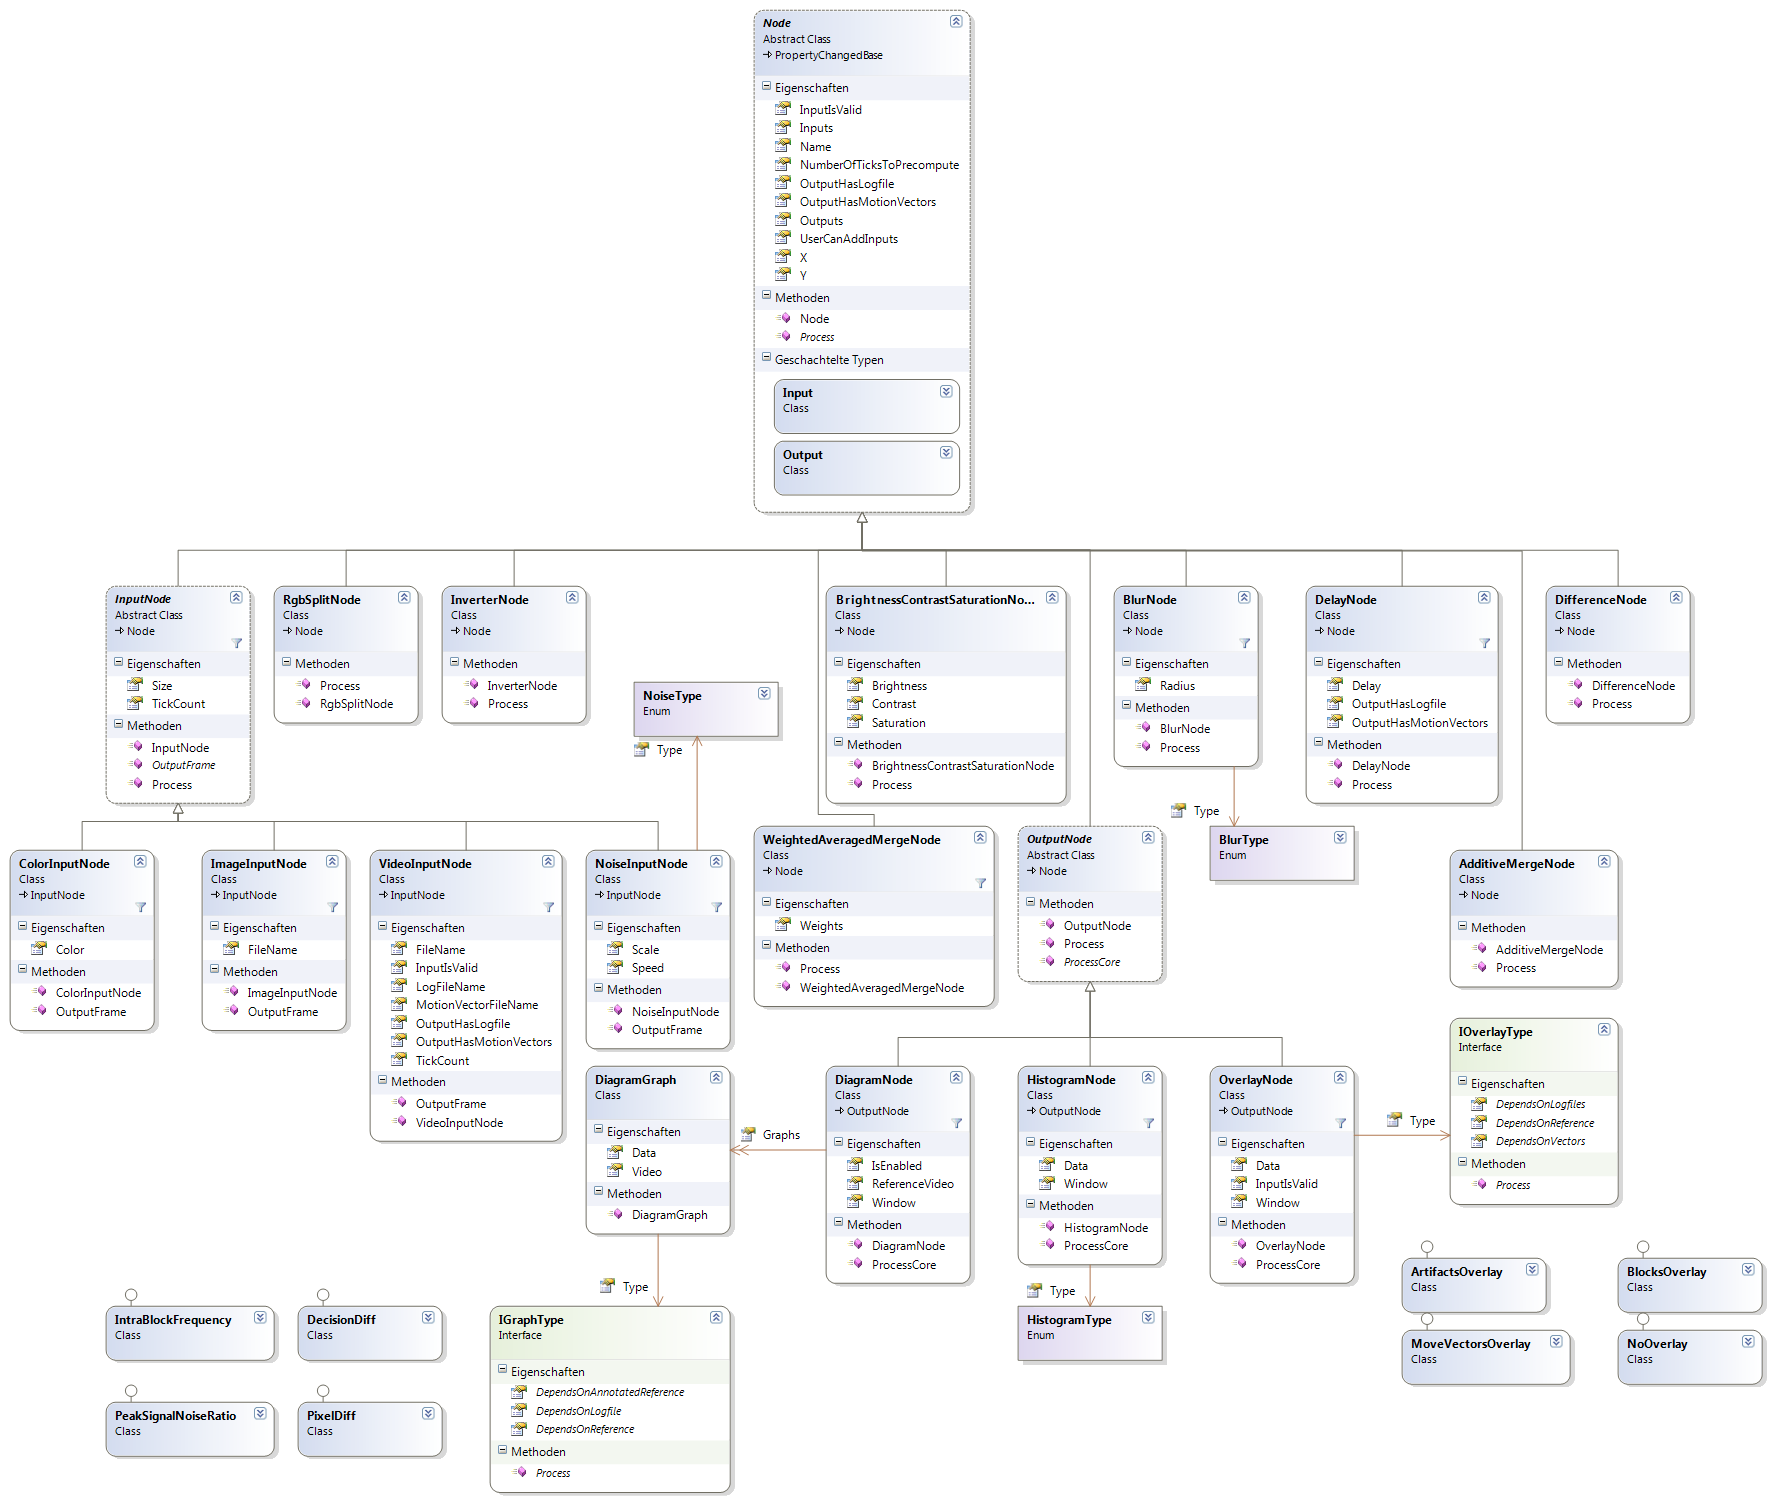
\includegraphics[width=0.8\textheight,angle=90]{classdiagram/pipe-imp.png}
\end{center}
\end{figure}
Namespace der vordefinierten Knotentypen. Diese werden dynamisch bei Programmstart ermittelt und geladen.
\newpage

\paragraph{\name{AveragedMergeNode}}
\begin{itemize}
	\change Wurde zu \name{WeightedAveragedMergeNode}  umbenannt, da es die Funktion des Knotens besser beschreibt.
\end{itemize}

\paragraph{\name{NoiseInputNode}}
\begin{itemize}
	\add \verb!public double? Scale { get; set; }! \\
	Diese neu eingeführte Option erlaubt es, dem Benutzer den angezeigten Perlin Noise zu skalieren.
	\add \verb!public double? Speed { get; set; }! \\
	Diese neu eingeführte Option erlaubt es, dem Benutzer die Geschwindigkeit des angezeigten Perlin Noise einzustellen.
\end{itemize}
Desweiteren wurden zwei neue Arten von Noise eingeführt, die Abwandlungen der schon existierenden sind (siehe \name{NoiseType}).

\paragraph{\name{NoiseType}}
\begin{itemize}
	\add \verb!ColoredCoherent! \\
	Erstellt farbigen Coherent Noise.
	\add \verb!ColoredPerlin! \\
	Erstellt farbigen Perlin Noise.
\end{itemize}

\paragraph{\name{DiagramGraph}}
\begin{itemize}
	\change \verb!public IList<KeyValuePair<int, double>> Data { get; set; }! \\
	Der Liste wurde jeweils der Tick des zugehörigen Analysedatums hinzugefügt.
\end{itemize}

\paragraph{\name{IGraphType}}
\begin{itemize}
	\add \verb!bool DependsOnAnnotatedReference { get; }! \\
	Ruft ab, ob der Diagrammtyp ein Referenzvideo mit Logfile benötigt.
	\add \verb!bool DependsOnLogfile { get; }! \\
	Ruft ab, ob der Diagrammtyp ein Logfile benötigt.
\end{itemize}

\paragraph{\name{HistogramNode}}
\begin{itemize}
	\change Die zur Berechnung des jeweiligen Histogrammtyps benötigten Methoden wurden als private Methoden ausgelagert.
\end{itemize}

\paragraph{\name{OverlayNode}}
\begin{itemize}
	\add \verb!public Frame Data { get; private set; }! \\
	Eine Schnittstelle, durch die andere Klassen das Resultat der Überlagerung abgreifen können. Dies ist notwendig, da die View die \name{Process}-Methode nicht selbst aufruft.
	\add \verb!public OverlayViewModel Window { get; }! \\
	Ruft das \name{OverlayViewModel}, welches zu diesem Knoten gehört, auf bzw. erstellt es. Dies ist notwendig, da die View wissen muss, dass dieser Knotentyp eine eigene Ausgabefensterart besitzt und sich dies mit einem entsprechenden \name{ProperyViewModel} ohne schwerwiegende Architektureingriffe sehr gut verwirklichen lässt.
\end{itemize}

\paragraph{\name{IOverlayType}}
\begin{itemize}
	\add \verb!bool DependsOnReference { get; }! \\
	Eine Wahrheitsvariable, die wiedergibt, ob die Überlagerungsart auf eine Referenz angewiesen ist.
	\add \verb!bool DependsOnVectors { get; }! \\
	Eine Wahrheitsvariable, die wiedergibt, ob die Überlagerungsart auf Bewegungsvektordaten angewiesen ist.
\end{itemize}

\paragraph{\name{+ NoOverlay}}~\\
Diese Klasse ist ein Überlagerungstyp, der nichts überlagert und somit stets verfügbar ist. Dies gilt unabhängig von den zusätzlichen Daten neben dem obligatorischen ursprünglichen Frame.
\newpage

\subsection{\name{YuvKA.ViewModel}}

\subsubsection*{Aktuelles Klassendiagramm}
\begin{figure}[h!]
\begin{center}
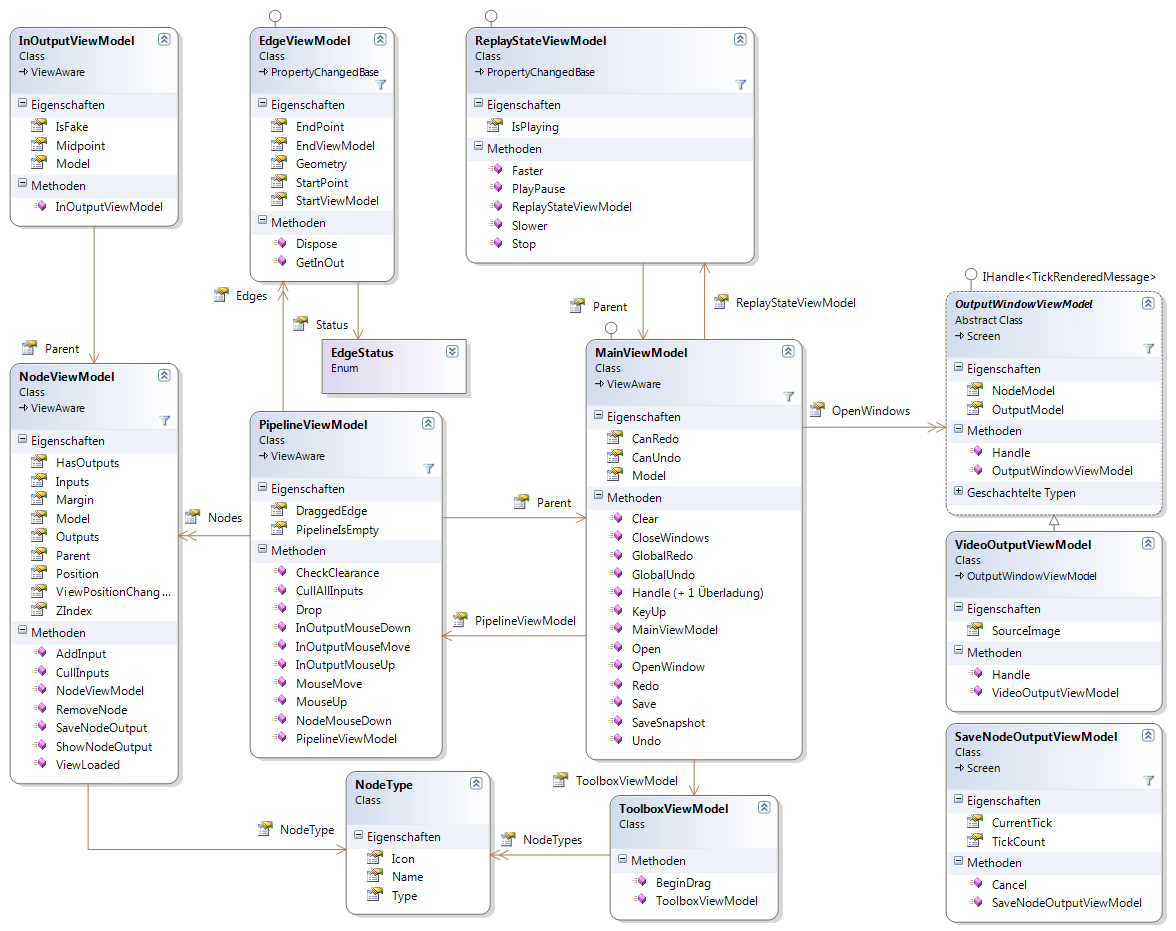
\includegraphics[width=\textwidth]{classdiagram/viewmodel.png}
\end{center}
\end{figure}
Nach dem MVVM-Pattern ist es Aufgabe der ViewModel-Schicht, der View das Model in einer für sie verarbeitbaren Form zu präsentieren. Bezogen auf das Projekt bedeutet dies vor allem, die Model-Klassen um View-spezifische Daten und Methoden zu ergänzen.
\newpage

Wie erwartet, hat sich im View Model eine große Anzahl an Änderungen ergeben, die zum Großteil aus dem Hinzufügen neuer Properties bestehen. Dies ist besonders der Tatsache geschuldet, dass das View Model nicht wirklich Teil der grundlegenden Architektur, sondern vielmehr Verknüpfungsschicht des Models und der View ist. Hierbei war die Architektur letztgenannter Schicht, nämlich WPF, bereits gegeben und  wurde wegen ihres unglaublichen Umfangs erst während der Implementierung Fall für Fall exakt erkundet. Deshalb werden im Weiteren die Änderungen beschrieben, ohne einzeln auf die Gründe einzugehen, warum von der Entwurfsarchitektur abgewichen wurde.

\paragraph{\name{EdgeViewModel}}
\begin{itemize}
	\add \verb!public InOutputViewModel StartViewModel { get; set; }! \\
	     \verb!public InOutputViewModel EndViewModel { get; set; }! \\
	Legt Anfang bzw. Ende der Kante auf einen Ein-/Ausgang fest. Nach Setzen der Properties werden Start- bzw. Endpunkt der Kante automatisch entsprechend aktualisiert.
	\add \begin{verbatim}public EdgeStatus Status { get; set; }
	enum EdgeStatus { Indeterminate, Invalid, Valid }
	\end{verbatim}
	Gibt während des Ziehens einer Kante ihren Zustand an, der in der View durch die Linienfarben weiß/rot/grün visualisiert wird.
	\add \verb!public void Dispose()! \\
	Entfernt alle Abonnements von Positionsänderungen der verbundenen Knoten, um Speicherlecks zu verhindern.
\end{itemize}

\paragraph{\name{+ InOutputViewModel}}~\\
Dies ist eine gemeinsames View Model für Inputs und Outputs.
\begin{itemize}
	\add \verb!public bool IsFake { get; }! \\
	Fake-Eingänge sind solche, ohne zugrundeliegendes Model. Sie werden für das dynamische Hinzufügen von Eingängen benötigt.
	\add \verb!public IObservable<Point> Midpoint { get; }! \\
	Gibt den jeweils aktuellen Mittelpunkt des Ein-/Ausgangs zurück.
	\add \verb!public object Model { get; }! \\
	Der zugrundeliegende Input oder Output
	\add \verb!public NodeViewModel Parent { get; }! \\
	Das View Model des Knotens dieses Ein-/Ausgangs
\end{itemize}

\paragraph{\name{MainViewModel}}
\begin{itemize}
	\add \verb!public void CloseWindows(Node node)! \\
	Erzwingt das Schließen aller Ausgabefenster dieses Knotens
	\add \verb!public void Handle(OutputWindowViewModel.ClosedMessage message)! \\
	Reagiert auf das Schließen eines Fensters.
	\add \verb!public void Handle(ChangeCommittedMessage message)! \\
	Reagiert auf in sich abgeschlossene Wertänderungen von Knoten-Properties.
\end{itemize}

\paragraph{\name{NodeViewModel}}
\begin{itemize}
	\add \verb!public bool HasOutputs { get; }! \\
	Gibt an, ob der Knoten derzeit Ausgänge besitzt.
	\add \verb!public IEnumerable<InOutputViewModel> Inputs { get; }! \\
	\verb!public IEnumerable<InOutputViewModel> Outputs { get; }! \\
	Wrappen die Ein-/Ausgänge des Knotens in enstprechende View Models.
	\add \verb!public Thickness Margin { get; }! \\
	Gibt die durch Position angegebene Verschiebung View-verträglich zurück.
	\add \verb!public Point Position { get; set; }! \\
	Zusammenfassung des X- und Y-Wertes des Knotens
	\add \verb!public IObservable<Unit> ViewPositionChanged { get; }! \\
	Beobachtbare Sequenz von Events, in der jeder Eintrag für die Veränderung der tatsächlichen Position auf der View steht.
	\add \verb!public int ZIndex { get; set; }! \\
	Regelt die Zeichenabfolge von Knoten, damit der letztausgewählte Knoten nicht von anderen verdeckt ist.
	\add \verb!public void AddInput()! \\
	Fügt bei dynamisch um Eingänge erweiterbaren Knoten einen neuen Eingang hinzu.
	\add \verb!public void CullInputs()! \\
	Führt CullInputs auf ViewModel-Ebene und anschießend im dargestellten Node aus.
	\add \verb!public void RemoveNode()! \\
	Entfernt diesen Knoten aus allen relevanten Listen und schließt alle Ausgabefenster des Knotens.
	\add \verb!public void ViewLoaded()! \\
	Eventhandler, um \name{ViewPositionChanged} initial zu triggern.
\end{itemize}

\paragraph{\name{NodeType}}
\begin{itemize}
	\add \verb!public string Name { get; set; }! \\
	Name des Knotens, der lesbarer ist als der reine Typname.
\end{itemize}

\paragraph{\name{PipelineViewModel}}
\begin{itemize}
	\add \verb!public EdgeViewModel DraggedEdge { get; }! \\
	Die gerade gezogene Kante, sonst null.
	\add \verb!public void CheckClearance(IDragEventInfo e)! \\
	Verhindert das Droppen eines Knoten, falls die Pipeline abgespielt wird.
	\add \verb!public void CullAllInputs()! \\
	In manchen Fällen, wie zum Beispiel beim Entfernen eines Knotens, ist es nötig die Eingänge aller Knoten des Graphen zu überprüfen und ggf. zu entfernen.
	\change \verb!public void Drop(IDragEventInfo e)! \\
	Der Parametertyp wurde von WPFs \verb!DragEventArgs! auf das eigens kreierte Interface \name{IDragEventInfo} geändert, da ersterer Typ nicht mockbar ist.
	\add \begin{verbatim}
public void InOutputMouseDown(InOutputViewModel inOut)
public void InOutputMouseMove(InOutputViewModel inOut,
    RoutedEventArgs e)
public void InOutputMouseUp(InOutputViewModel inOut)
public void MouseMove(IMouseEventInfo e)
public void MouseUp()
public void NodeMouseDown(NodeViewModel inOut, IMouseEventInfo e)
	\end{verbatim}
	Eventhandler für Drag \& Drop
\end{itemize}

\paragraph{\name{ReplayStateViewModel}}
\begin{itemize}
	\remove \verb!public bool IsPlaying { get; }! \\
	Verschoben in \name{PipelineState}, damit dort der gesamte Wiedergabezustand gehalten wird.
\end{itemize}

\paragraph{\name{VideoOutputViewModel}}
\begin{itemize}
	\add \verb!public WriteableBitmap SourceImage { get; }! \\
	Speichert das Bild, das als nächstes in das Ausgabefenster gezeichnet werden soll.
\end{itemize}
\newpage

\subsection{\name{YuvKA.ViewModel.Implementation}}

\subsubsection*{Aktuelles Klassendiagramm}
\begin{figure}[h!]
\begin{center}
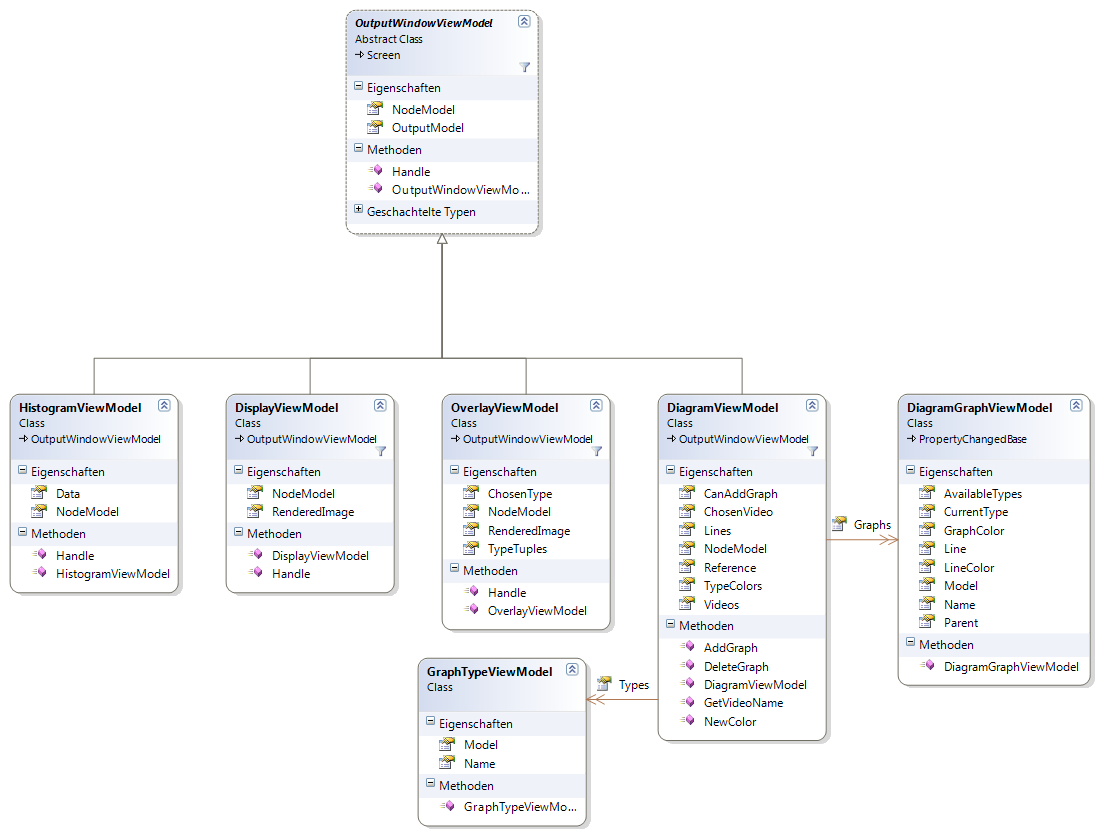
\includegraphics[width=\textwidth]{classdiagram/viewmodel-imp.png}
\end{center}
\end{figure}
Namespace der ViewModels der vordefinierten Knotentypen.
\newpage

\paragraph{\name{HistogramViewModel}}
\begin{itemize}
	\add \begin{verbatim}public EnumerableDataSource<KeyValuePair<int, double>> Data {
    get; }\end{verbatim} \\
	Ruft die Analysedaten des Histogrammes ab oder setzt diese fest.
\end{itemize}

\paragraph{\name{DiagramViewModel}}
\begin{itemize}
	\add \verb!public Tuple<string, Node.Input> Reference { get; set; }! \\
	Ruft das Referenzvideo des Diagrammknotens ab oder setzt dieses fest.
	\add \verb!public IEnumerable<Tuple<string, Node.Input>> Videos { get; }! \\
	Ruft die Eingabevideos des Diagrammknotens ab und fügt diesen einen Index hinzu.
	\add \verb!public Tuple<string, Node.Input> ChosenVideo { get; set; }! \\
	Ruft das aktuell vom Benutzer zur Analyse ausgewählte Video ab oder setzt dieses fest.
	\add \verb!public ObservableCollection<DiagramGraphViewModel> Graphs { get; }! \\
	Ruft die Graphen des Diagramms ab.
		\add \verb!public IEnumerable<LineGraph> Lines { get; }! \\
	Ruft die Kurven im Diagramm ab, die den Graphen des Diagrammknotens entsprechen. 
	\add \verb!public bool CanAddGraph { get; }! \\
	Ruft ab, ob ein neuer Graph hinzugefügt werden kann.
	\change \verb!public void AddGraph()! \\
	Der Node.Input-Parameter wurde entfernt, diese Funktion wurde von ChosenVideo übernommen.
	\add \verb!public System.Windows.Media.Color NewColor(IGraphType type)! \\
	Erzeugt eine neue Farbe, die vom Grundfarbton des angegebenen IGraphTypes abgeleitet wird.
	\add \verb!public string GetVideoName(Node.Input input)! \\
	Gibt den Namen eines Eingabevideos zurück, der aus seinem Index und seinem Quellknoten erzeugt wird.
\end{itemize}

\paragraph{\name{+ DiagramGraphViewModel}}~\\
Repräsentiert das Objekt, mit dem die Einstellungen des Graphen im Ausgabefenster verwaltet werden.
\begin{itemize}
	\add \verb!public DiagramViewModel Parent { get; }! \\
	Ruft das DiagramViewModel, das diesem DiagramGraphViewModel zugrunde liegt, ab.
	
	\add \verb!public DiagramGraph Model { get; }! \\
	Ruft den Diagrammgraphen ab oder setzt ihn fest.
	\add \verb!public string Name { get; }! \\
	Ruft den Namen des Videos des Graphen ab.
	\add \verb!public IEnumerable<GraphTypeViewModel> AvailableTypes { get; }! \\
	Ruft die mit den momentanen Einstellungen verfügbaren Graphentypen ab.
	\add \verb!public GraphTypeViewModel CurrentType { get; set; }! \\
	Ruft den momentan vom Benutzer gewählten Graphentypen ab oder setzt ihn fest.
	\add \verb!public IEnumerable<GraphTypeViewModel> AvailableTypes { get; }! \\
	Ruft alle verfügbaren Graphentypen ab.
	\add \verb!public LineGraph Line { get; }! \\
	Ruft die Kurve des Diagrammgraphen ab.
	\add \verb!public Color LineColor { get; }! \\
	Ruft die momentan verwendete Farbe für die Kurve ab.
	\add \verb!public SolidColorBrush GraphColor { get; }! \\
	Ruft die Farbe für die Vorschau der Kurve ab.
\end{itemize}

\paragraph{\name{+ GraphTypeViewModel}}~\\
Repräsentiert das Objekt, mit dem die Graphentypen im Ausgabefenster angezeigt werden.
\begin{itemize}
	\add \verb!public IGraphType Model { get; }! \\
	Ruft den GraphenTypen ab.
	\add \verb!public string Name { get; }! \\
	Ruft den Namen des GraphenTypen ab.
\end{itemize}

\paragraph{\name{+ HslHelper}}~\\
Enthält eine Methode zur Konvertierung zwischen dem HSL- und dem RGB-Farbraum, sodass sie von mehreren Klassen verwendet werden kann.
\begin{itemize}
	\add \verb!public static Color HslToRgb(double h, double s, double l)! \\
	Konvertiert eine Farbe vom HSL-Farbraum zum RGB-Farbraum.
\end{itemize}

\paragraph{\name{OverlayViewModel}}
\begin{itemize}
	\add \verb!public System.Tuple<string, IOverlayType> ChosenType { get; set; }! \\
	Ein Tupel, welches den Namen und den Typ des gerade verwendeten Überlagerungstyps enthält.
	\add \verb!public WriteableBitmap RenderedImage { get; }! \\
	Das Ergebnis der Überlagerung für die View aufbereitet. Dies ist notwendig, da die View einen \name{Frame} nicht ohne weiteres darstellen kann.
	\add \begin{verbatim}public IEnumerable<System.Tuple<string, IOverlayType>>
	     TypeTuples { get; }
	     \end{verbatim}
	Eine Sammlung aller momentan verfügbaren Überlagerungstypen in Form von Tupeln mit Namen und Typ. Dies ist notwendig für die View, um die Auswahl der Überlagerungen darzustellen.
\end{itemize}
\newpage

\subsection{\name{YuvKA.ViewModel.PropertyEditor}}

\subsubsection*{Aktuelles Klassendiagramm}
\begin{figure}[h!]
\begin{center}
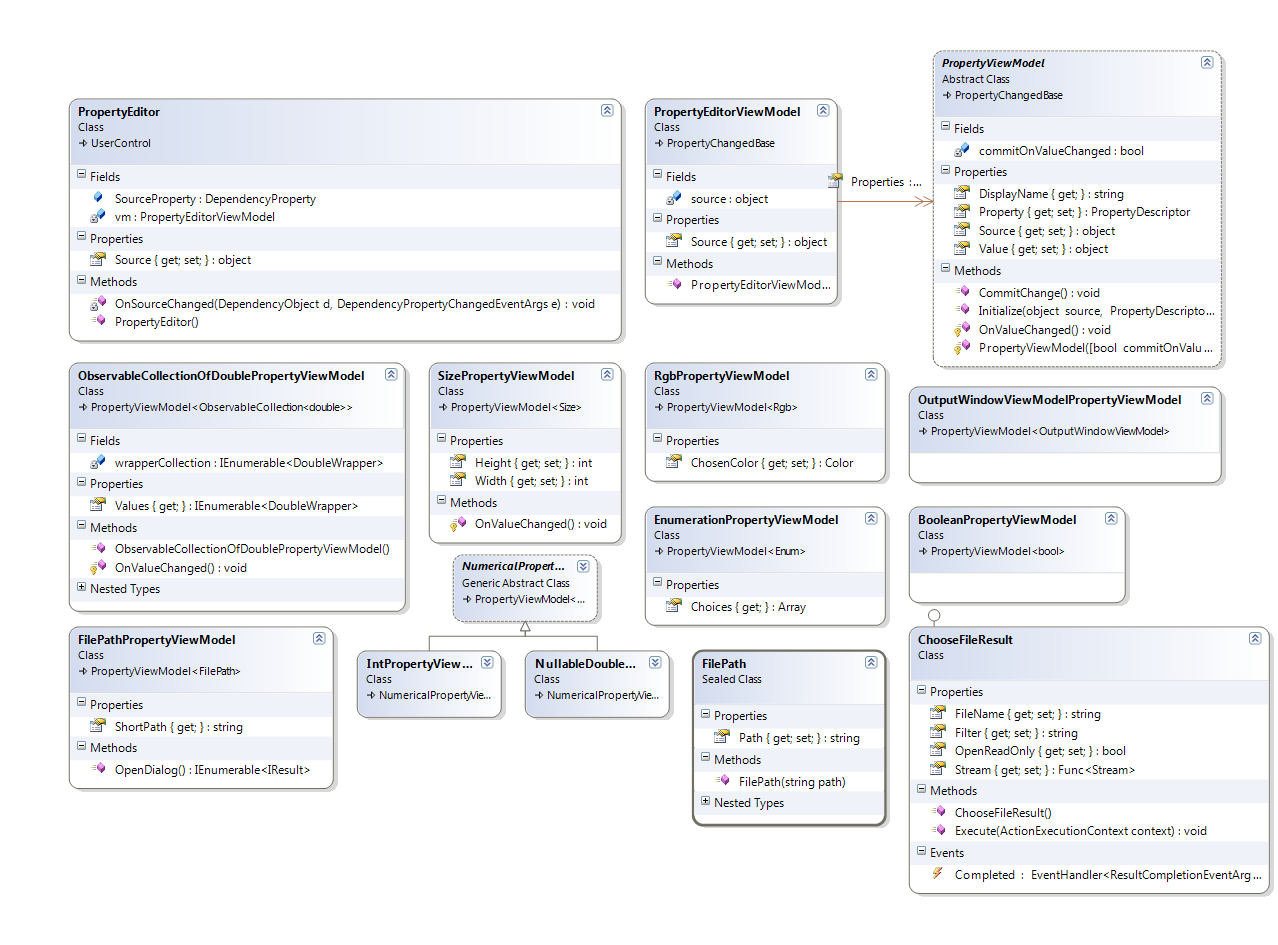
\includegraphics[width=\textwidth]{classdiagram/propertyeditorvm.png}
\end{center}
\end{figure}
Die Klassen des PropertyEditor-Namespaces erzeugen für ein beliebiges Objekt dynamisch eine Oberfläche zum Anzeigen und Ändern seiner Property-Werte. Die Menge der darstellbaren Property-Typen ist dynamisch erweiterbar.
\newpage

\paragraph{\name{PropertyViewModel}}
\begin{itemize}
	\add \verb!public string DisplayName { get; }! \\
	Gibt das \name{DescriptionAttribute} der Property bzw. den Namen der Property weiter. Dies ist notwendig, um der View deskriptivere Namen der Properties bereitzustellen.
	\add \verb!public void CommitChange()! \\
	Diese Methode benachrichtigt alle anderen Objekte, dass sich diese Property geändert hat. Dies ist notwendig, damit ein Undo-Schritt erstellt werden kann.
	\add \verb!public void Initialize(object source, PropertyDescriptor property)! \\
	Diese Methode weist einem PropertyViewModel eine Property und die Quelle der Property zur Verwaltung zu. Dies ist notwendig, da das PropertyViewModel einen argumentlosen Konstruktor benötigt und sich nur auf diese Weise sicherstellen lässt, dass die Property und deren Quelle immer gemeinsam gesetzt werden.
\end{itemize}

\paragraph{\name{PropertyViewModel<T>}}
\begin{itemize}
	\change \verb!public T TypedValue { get; set; }! \\
	Der typisierte Wert der Property wurde umbenannt, um Namenskonflikte mit dem untypisierten Wert der Property der Oberklasse zu vermeiden.
\end{itemize}

\subsection{\name{YuvKA.ViewModel.PropertyEditor.Implementation}}

\paragraph{\name{DoublePropertyViewModel}}
\begin{itemize}
	\change Wurde zu \name{NullableDoublePropertyViewModel} umbenannt, da der zugrundeliegende Typ zu \name{Nullable<double>} geändert wurde.
	\add \verb!public bool SlidersAreEnabled { get; }! \\
	Ruft ab, ob der zugrundeliegende Wert gültig ist und der in der UI dargestellte Slider als Folge dessen aktiviert sein soll oder nicht.
\end{itemize}

\paragraph{\name{NumericalPropertyViewModel}}
\begin{itemize}
	\change \verb!public double Maximum { get; }! \\
	Die \name{Maximum}-Property wurde auf read-only gesetzt.
	\change \verb!public double Minimum { get; }! \\
	Die \name{Minimum}-Property wurde auf read-only gesetzt.
\end{itemize}

\paragraph{\name{ObservableCollectionOfDoublePropertyViewModel}}
\begin{itemize}
	\add \verb!public IEnumerable<DoubleWrapper> Values! \\
	\name{IEnumerable} des neu eingeführten Typs \name{DoubleWrapper}. Wurde eingeführt, um Data Binding von der Benutzeroberfläche her zu ermöglichen.
	\add \verb!public class DoubleWrapper! \\
	Innere Wrapper-Klasse um einen \name{double}-Wert herum. Diese wird benötigt, um von der View aus per Data Binding auf den Wert des double zuzugreifen.
\end{itemize}

\paragraph{\name{+ OutputWindowViewModelPropertyViewModel}}~\\
Erlaubt es Wiedergabeknoten, beliebige ViewModels selbst zu liefern, welche dann vom Programm gelesen und angezeigt werden.

\paragraph{\name{RgbPropertyViewModel}}
\begin{itemize}
	\change Da \name{Rgb} nicht serialisierbar war, wurde es durch \name{Color} ersetzt und in logischer Konsequenz dieses View Model zu \name{ColorPropertyViewModel} umbenannt.
	\remove \verb!public bool OpenDialog()! \\
	Die \name{OpenDialog}-Methode wurde entfernt, da das Projekt jetzt den \name{ColorPicker2} aus dem \name{PropertyTools.Wpf}-Projekt benutzt
	\add \verb!public Color ChosenColor { get; set; }! \\
	Stellt eine Property für die vom Benutzer gewählte Farbe bereit.
\end{itemize}
\newpage

\subsection*{Fazit}

Die Implementation hat gezeigt, dass der ursprüngliche Architekturentwurf zum großen Teil eingehalten wurde. In den im Entwurf festgelegten Klassen gab es kaum Veränderungen, es wurden lediglich weitere Properties oder Methoden hinzugefügt, die sich erst in der Implementation als notwendig erwiesen. Eine Ausnahme hiervon ist das View Model, dessen Klassen teilweise 
komplett geändert wurden. Dies lag auch unter anderem daran, dass Frameworks verwendet wurden (z.B. im \name{DiagramViewModel} zum Zeichnen der Diagramme), die erst in der Implementierung ausgewählt wurden, sodass die Klassen entsprechend angepasst werden mussten.
